\chapter{Implementation}

This is an overview of the implementation process and how the product evolved throughout the project. In addition to this chapter, the status reports can be found in the appendix. \\

\section{Iteration 1}

Week 5 - 8\\
\newline
In this period, most of the time was spent on research, learning, and gathering and clarifying the requirements. The group lacked extensive experience with JavaScript and Node.js, so it was necessary to spend the first weeks on getting to know these technologies. Translating the requirements of a board game into a version that would work in an electronic format also took a significant amount of time in those weeks.\\
\newline
Week 8 - 9\\
\newline
The first version of the user interface, and a barebones server was implemented in the next few weeks. Algorithms for constructing nodes, zones and paths, as well as proper listening functions for moving and selecting objects were developed.\\

%Initial interface
\begin{figure}[H]
  \centering
    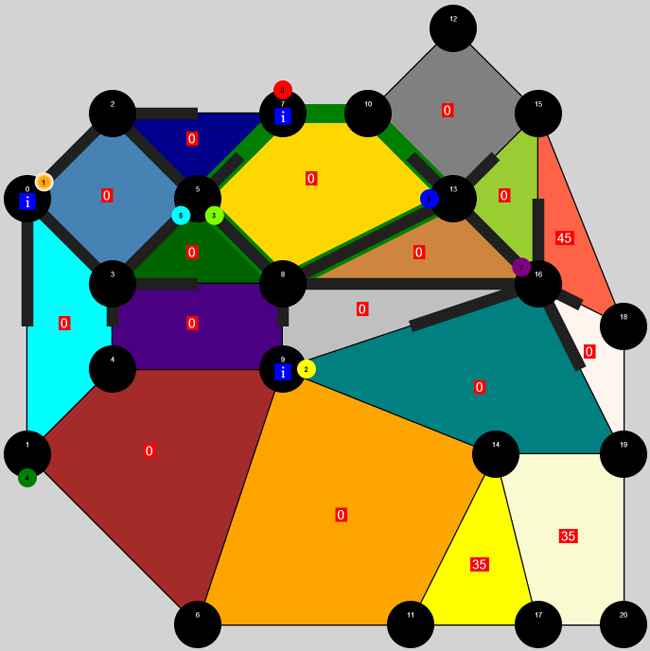
\includegraphics[width=1.0\textwidth]{img/canvas.png}
  \caption{User interface, 'First Iteraton'} 
  \label{fig:canvas}
\end{figure}


\section{Iteration 2}

Week 10 - 14\\
\newline
In iteration 2, the server was in focus, and was populated with most of the core game functionality (FR5) such as moving players, decreasing panic, info cards and events, and timer. Sidebars for player information was added, as well as a status bar showing relevant information with buttons to execute actions on selected items.\\

% FIG better interface
\begin{figure}[H]
  \centering
    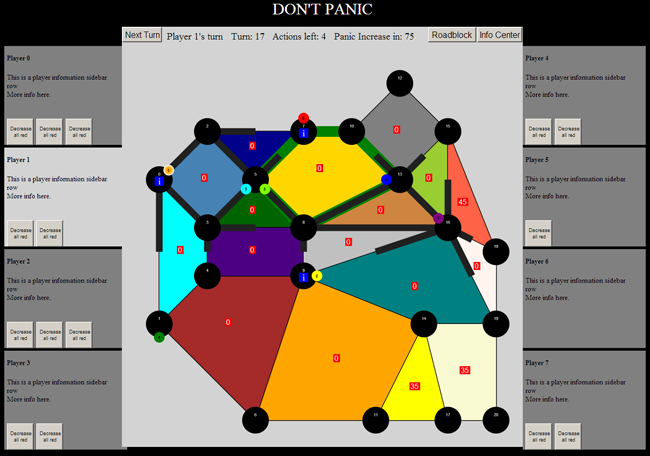
\includegraphics[width=1.0\textwidth]{img/earlyVersion.png}
  \caption{User interface, ' User interface with players, cards and status bar'} 
  \label{fig:earlyversion}
\end{figure}

\section{Iteration 3}

Week 15 - 18\\
\newline
The third iteration was focused on the functionality outside the game. The expert interface was created, which creates game templates and maps that can be loaded into the game. The website got an index page, and general website functionality so users can navigate between the pages easily.\\

\begin{figure}[H]
  \centering
    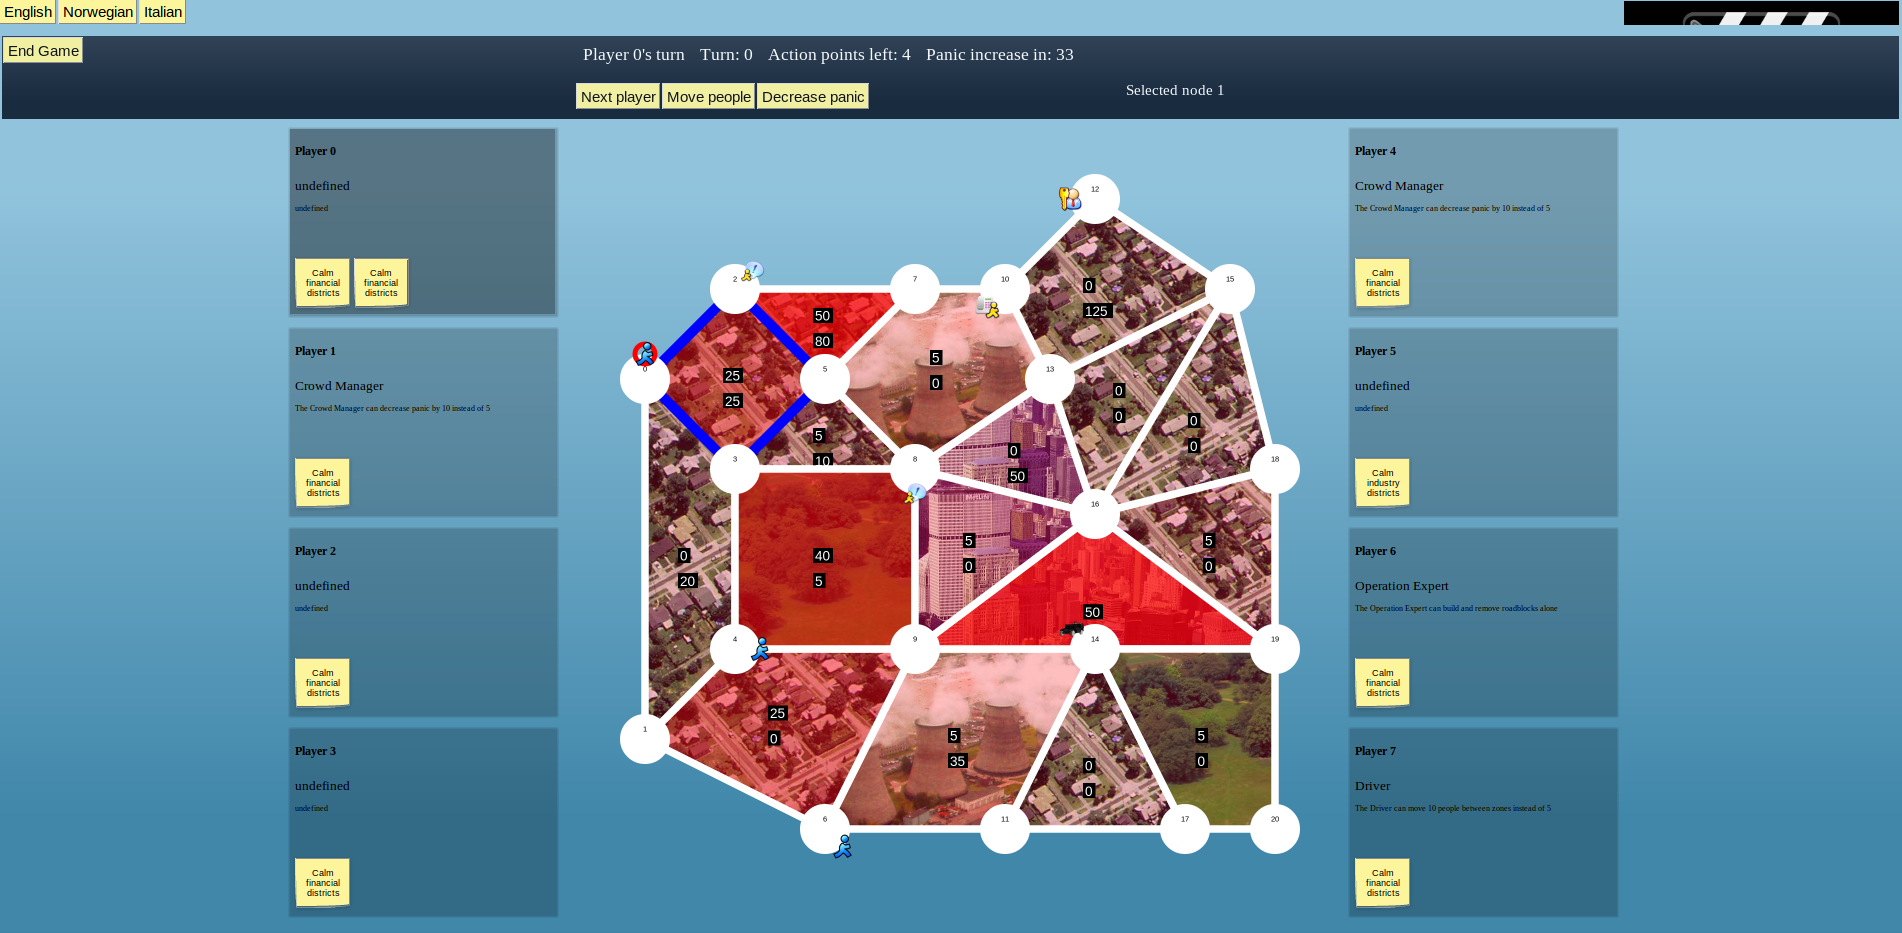
\includegraphics[width=1.0\textwidth]{img/gamefinal.png}
  \caption{Game Interface, 'Final version'} 
  \label{fig:gamefinal}
\end{figure}
% FIG expert interface

\begin{figure}[H]
  \centering
    \includegraphics[width=1.0\textwidth]{img/ExpertInterfaceForm.png}
  \caption{Expert Interface, 'Final version'} 
  \label{fig:EcpertInterfaceForm}
\end{figure}
% FIG expert interface


\begin{figure}[H]
  \centering
    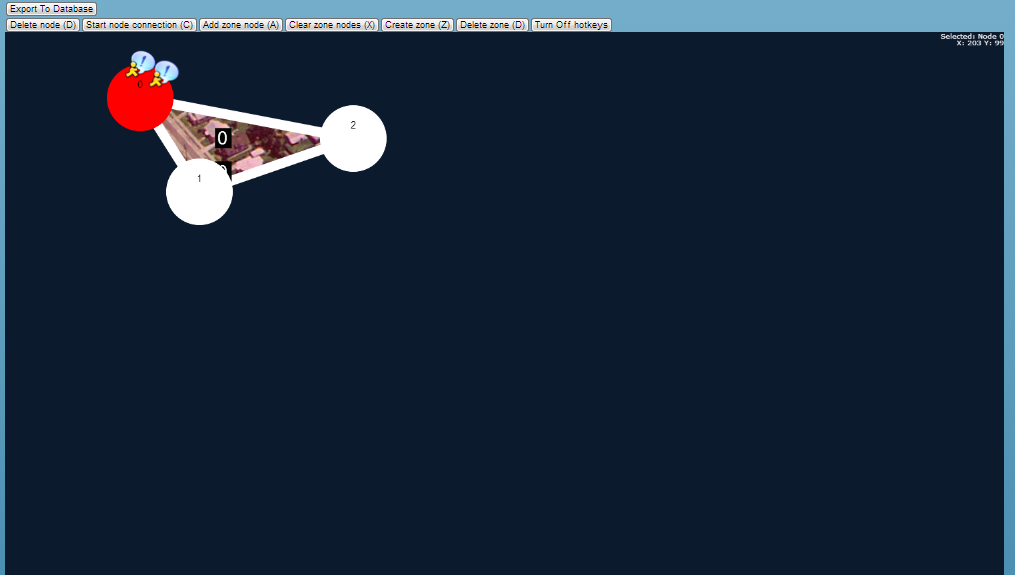
\includegraphics[width=1.0\textwidth]{img/ExpertInterfaceCanvas.png}
  \caption{Expert Interface Map Creation, 'Final version'} 
  \label{fig:EcpertInterfaceCanvas}
\end{figure}
% FIG expert interface

\section{Iteration 4}

Week 18 - 19\\
\newline
The last few weeks of coding were spent on stabilizing the codebase, as well as adding more complicated features that had been worked on for some time, like the ability to watch replays of games that have been played, the Game Master interface which enables an expert to watch a game in progress and take control of players, and the ability to translate the game and website into other languages.\\


%FIG replay, index in norwegian and english

\begin{figure}[H]
  \centering
    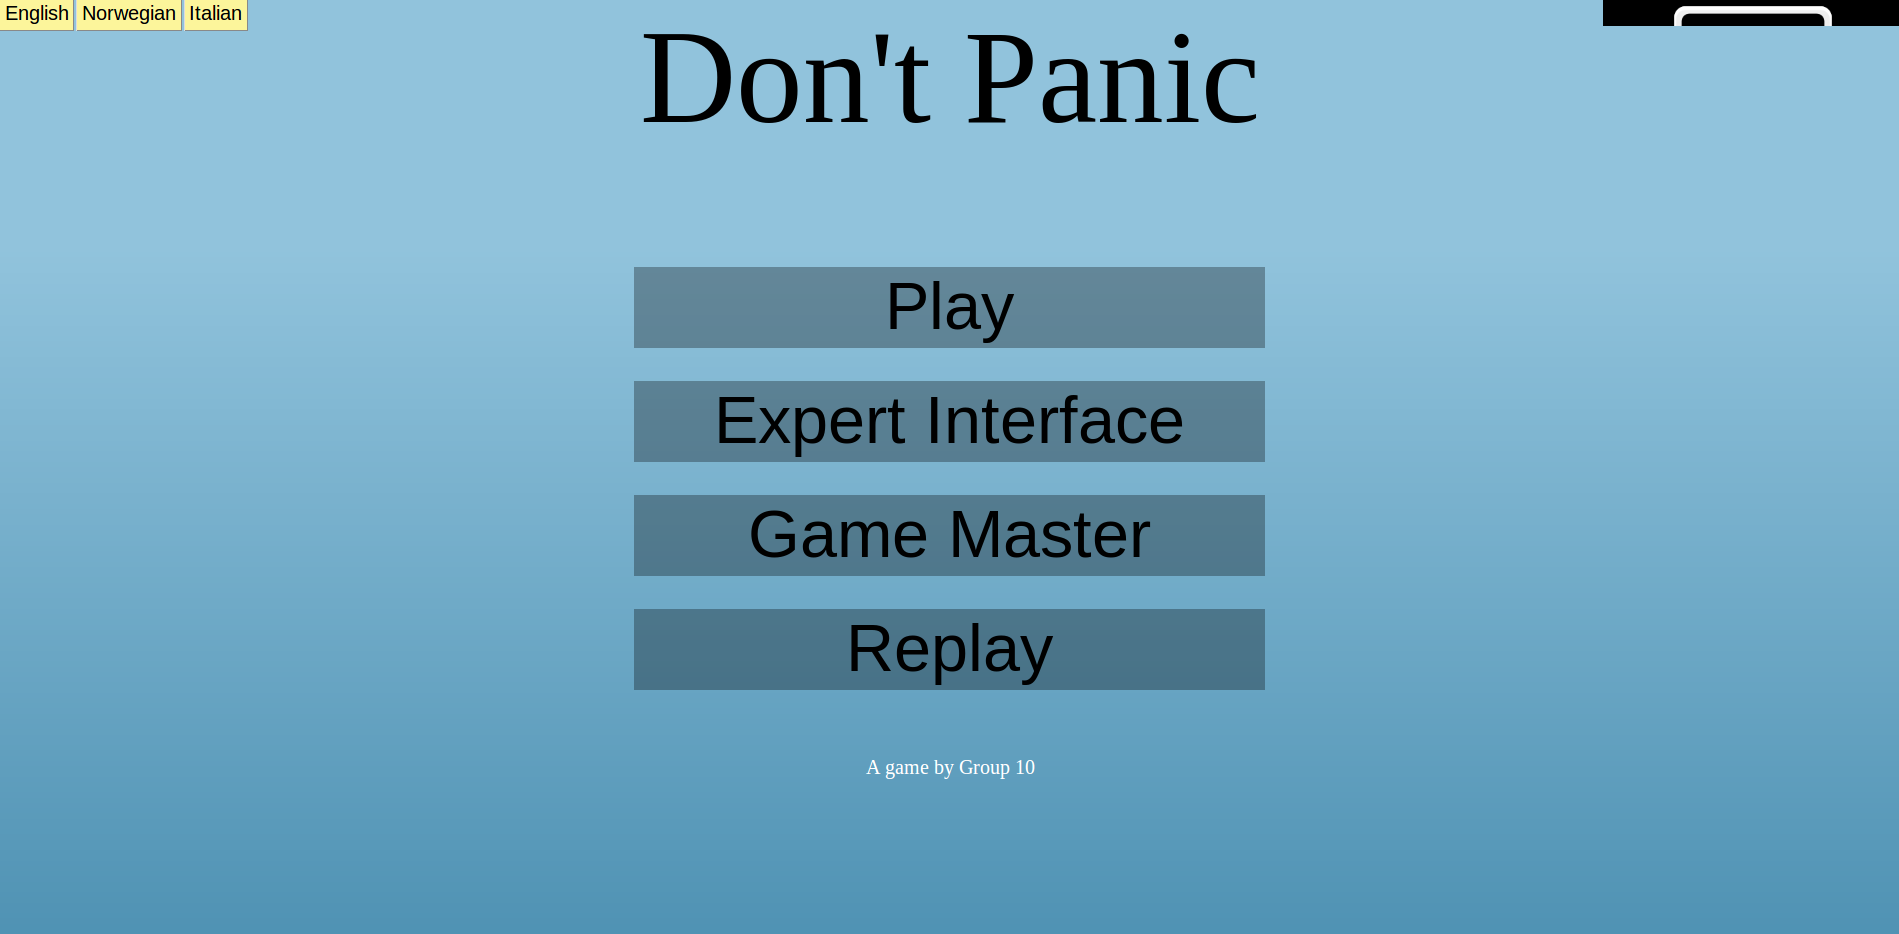
\includegraphics[width=1.0\textwidth]{img/indexen.png}
  \caption{Index, ' Index page in english'} 
  \label{fig:indexen}
\end{figure}

\begin{figure}[H]
  \centering
    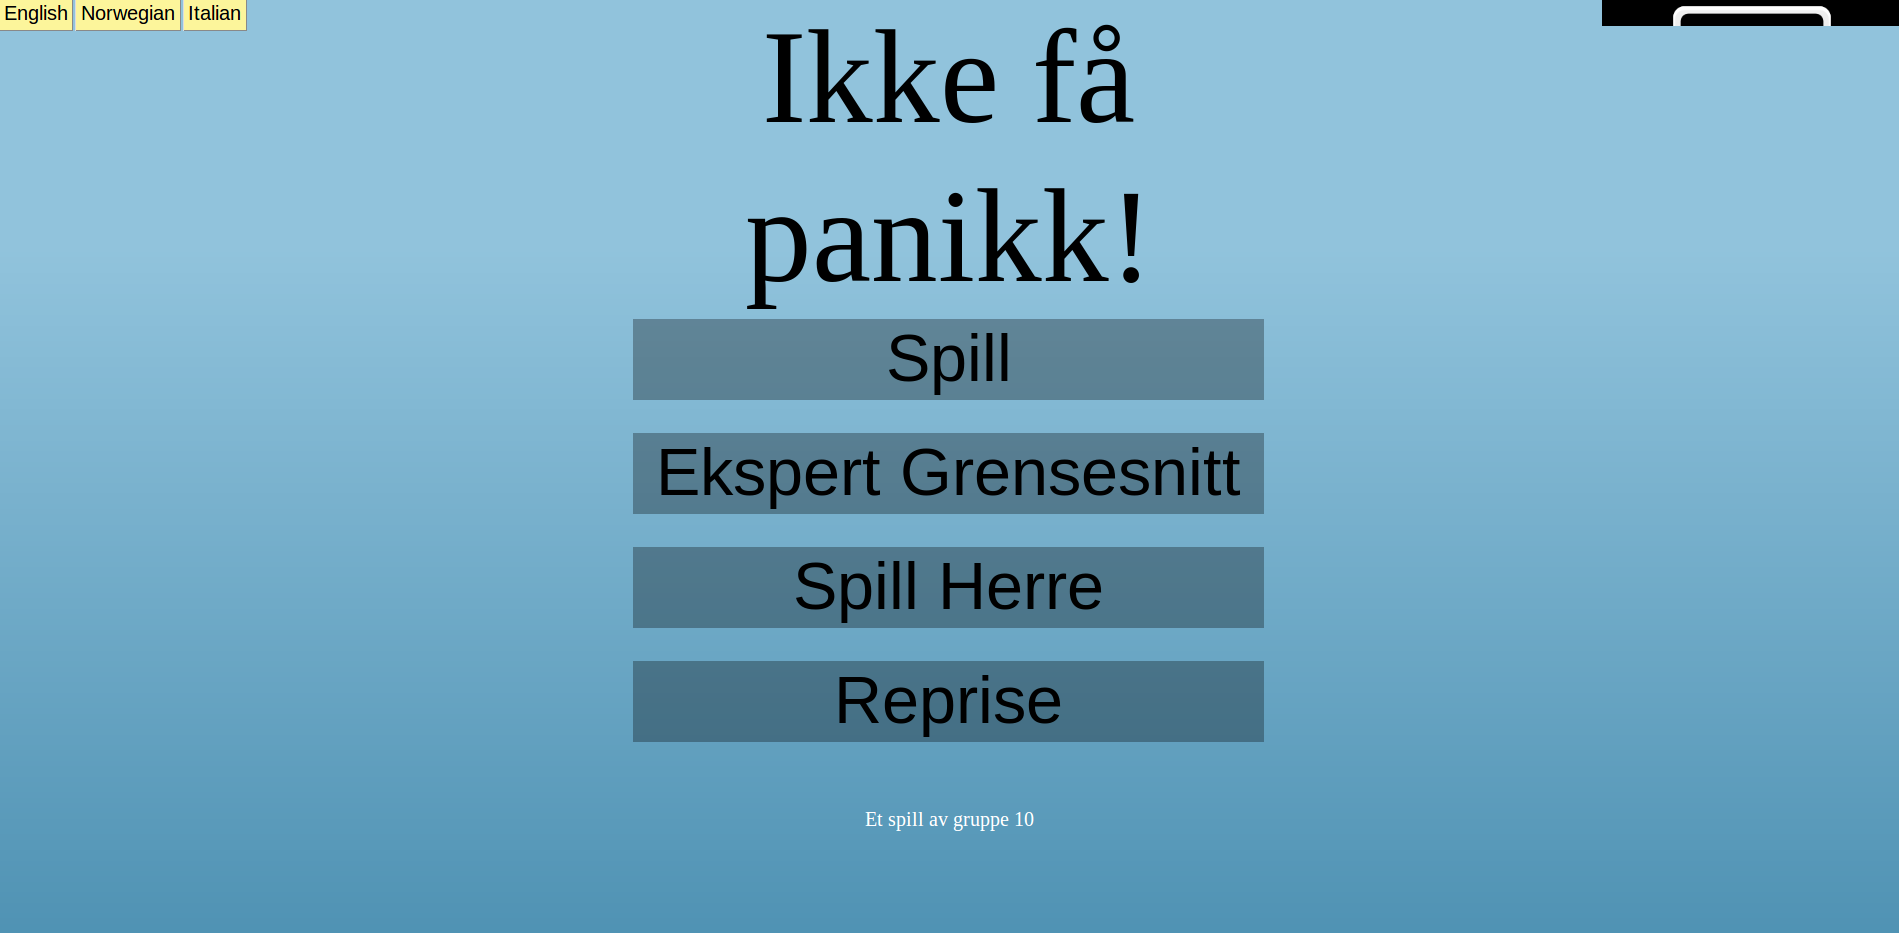
\includegraphics[width=1.0\textwidth]{img/indexno.png}
  \caption{Index, ' Index page in norwegian'} 
  \label{fig:indexno}
\end{figure}


